\section{서론}
\label{sec:intro}

% [문단 1: 문제 정의 — Few-shot 배경 및 High-Score Ambiguity 정의]
다품종 소량 생산과 잦은 라인 전환이 일어나는 제조 현장에서는 제품마다 결함 데이터를 충분히 모으거나 모델을 다시 학습하기 어려워, 소수의 정상 이미지만으로 결함 위치를 찾는 few-shot 이상 국소화가 실용적인 대안이 된다.
대표적인 방식은 동결된 사전학습 백본~\cite{dinov2}에서 추출한 정상 패치 특징으로 참조 뱅크를 만들고, 쿼리 패치와의 최근접 거리를 이상 점수로 쓰는 것이다~\cite{patchcore,anomalydino,superad}.
이 점수는 정상 쿼리 패치라면 참조 뱅크 안에 가까운 이웃이 있다는 가정에 기댄다.
그러나 실제 공정에서는 조명 드리프트, 부품 자세 변동, 표면 난반사 같은 획득 조건 변화가 계속 발생하며~\cite{aebad,mvtecad2}, 몇 장의 정상 서포트로는 이를 모두 담을 수 없다.
서포트에 없는 정상 변동이 나타나면 결함이 없는 패치도 최근접 거리가 커지고, 이 값은 실제 결함이 만든 큰 거리와 같은 구간에 놓일 수 있다.
따라서 큰 거리값만으로는 그 원인이 결함인지 서포트에 없던 정상 외관 변화인지 확정할 수 없으며, 본 논문은 이를 \textbf{High-Score Ambiguity}라 부른다(\cref{fig:intro-ambiguity}).
이 모호성은 오경보를 엄격히 제한하는 저-FPR 구간에서 특히 문제가 되는데, 정상 위치의 고점수로 인한 오경보를 줄이려고 판정 임계값을 높이면 함께 검출할 수 있는 결함 영역도 줄어들기 때문이다~\cite{aupimo}.

\begin{figure}[t]
\centering
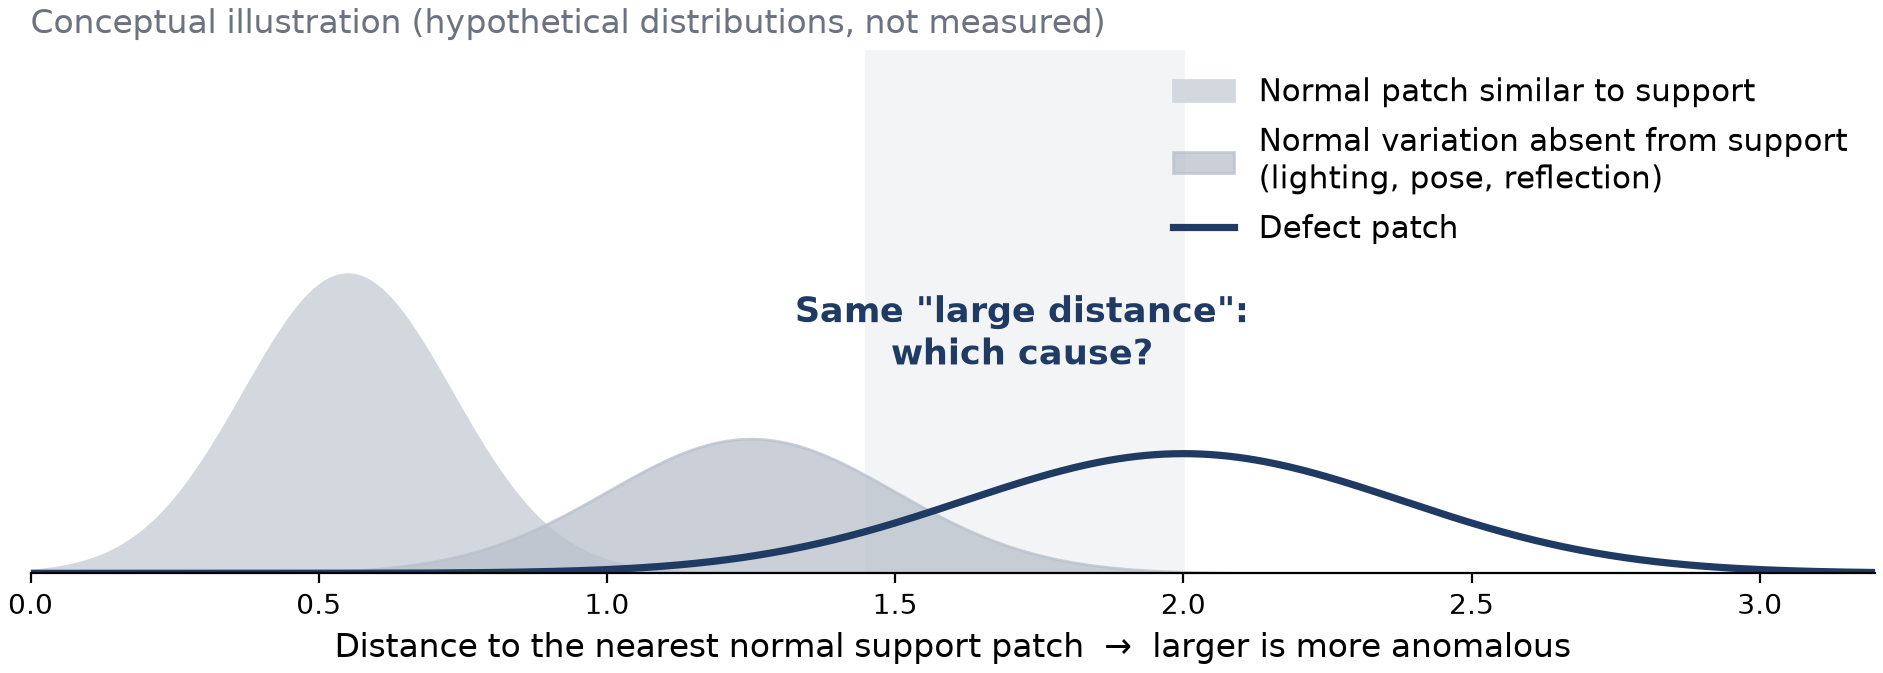
\includegraphics[width=\linewidth]{figures/fig_intro_ambiguity.png}
\caption{\textbf{Conceptual illustration of High-Score Ambiguity in few-shot inspection.} With sparse normal support, unobserved normal variations and true defects can both produce large nearest-neighbor distances. Raising the decision threshold to limit false alarms from normal high scores can also reduce defect coverage.}
\label{fig:intro-ambiguity}
\end{figure}

% [문단 2: 접근 방향 제안 — 계층·해상도 관측 확장 및 개별 매칭]
정상 서포트를 충분히 확보하면 더 다양한 정상 외관을 참조 뱅크에 담을 수 있지만, few-shot 조건에서는 사용할 수 있는 이미지 수가 제한된다.
따라서 한정된 서포트에서 결함 판단에 쓸 수 있는 시각적 단서를 충분히 확보하는 것이 중요하다.
본 논문은 이를 위해 표현 계층과 입력 해상도의 두 축으로 관측을 확장하되, 다층 특징을 단일 벡터로 묶어 하나의 이웃만 찾는 기존 접근~\cite{patchcore}과 달리 각 계층·해상도를 독립된 매칭 단위로 분리하는 방향을 취한다.
ViT는 계층마다 국소 외관과 전역 문맥을 반영하는 방식이 다르므로, 여러 계층의 특징은 서로 다른 수준의 비교 단서를 제공한다~\cite{raghu2021vision,ranftl2021vision}.
또한 입력 해상도는 각 패치가 나타내는 원본 영상의 공간 범위를 바꾸며, 패치 크기가 고정된 백본에서는 해상도가 높을수록 더 작은 영역이 하나의 토큰에 대응한다~\cite{shi2024scaling,fu2024featup}.
따라서 여러 계층과 해상도에서 참조 매칭을 개별적으로 수행하면, 미세한 국소 차이와 더 넓은 영역의 문맥적 차이를 각자의 표현·공간 척도에서 독립적인 비교 단서로 확보할 수 있다.

% [문단 3: 구체적인 문제 — 다관측 거리 통합 시의 척도 불균형과 오경보 유입]
그러나 이렇게 분리하여 확보한 다관측 매칭 거리를 하나의 이상 점수로 통합할 때, 원시 거리를 단순 합산하거나 평균하면 두 가지 구체적인 문제가 발생한다. 
첫째, 계층의 깊이와 입력 해상도에 따라 정상 참조 거리가 형성하는 기본 분포의 척도가 서로 다르므로, 보정 없이 동일한 계수를 적용하면 평소 거리 값이 큰 특정 관측이 최종 이상 점수를 일방적으로 지배하여 결합 결과가 왜곡된다. 
둘째, 관측 간 거리 척도를 맞추더라도 모든 계층을 동등한 비중으로 결합하면 계층별 민감도 차이로 인한 한계가 나타난다. 
얕은 계층의 특징은 미세한 국소 결함을 포착하는 데 유리하지만 조명이나 표면 질감 같은 정상 외관 변화에도 민감하게 반응하는 반면, 깊은 계층은 전역 문맥을 바탕으로 정상 변이에 비교적 강건하다. 
따라서 계층별 특성을 구분하지 않고 점수를 합치면, 얕은 계층에서 발생한 정상 변이의 큰 거리가 결합 점수에 그대로 유입되어 저-FPR 구간에서의 오경보(High-Score Ambiguity)를 다시 악화시킨다. 
결국 다관측 통합이 유효하려면 관측 간 거리 단위의 불균형과 계층별 오경보 민감도 차이를 동시에 해결해야 한다.

% [문단 4: 해결 방안 — ScopeAD (정상 참조 기반 선형 결합)]
이를 해결하기 위해 본 논문은 다관측 확장과 정상 참조 기반 선형 결합(Support-Referenced Linear Fusion)으로 구성된 \textbf{\method}를 제안한다. 
\method는 계층·해상도별 독립 뱅크에서 산출한 매칭 거리를 통합할 때, 단순 이상 맵 평균~\cite{superad}이나 단일 스케일 보정~\cite{freepatch}과 달리 관측별 정상 참조 척도와 계층별 고정 가중치를 함께 사용하여 선형 결합 계수를 정의한다. 
구체적으로 각 관측의 정상 서포트 내부 거리 분포로부터 기준 단위를 추정해 관측 간 척도를 정규화한 뒤, 깊은 계층의 정규화 점수 평균에 얕은 계층의 정규화 점수를 작은 고정 가중치로 더한다. 
이 선형 결합을 각 해상도에 적용한 후, 해상도별 맵을 원본 좌표에서 평균하여 최종 이상 맵을 생성한다. 
\method는 백본의 추가 학습이나 쿼리 시점 파라미터 갱신 없이 동작하며, 계층 가중치는 개발 평가에서 한 번 정한 뒤 모든 데이터셋과 shot 조건에 고정한다.

본 논문의 기여는 다음과 같다.
\begin{itemize}
  \item 제한된 정상 서포트에서 다양한 비교 단서를 활용하도록, 동결 백본의 계층·입력 해상도를 확장하고 관측별 매칭 거리를 독립적으로 유지하는 few-shot 이상 국소화 방법을 구성한다.
  \item 정상 서포트에서 추정한 기준 척도와 계층별 고정 가중치를 함께 사용하여 관측별 결합 계수를 정의하는 정상 참조 기반 선형 결합을 제안한다.
  \item 관측 구성과 결합 대안에 대한 비교로 전체 설계의 효과와 한계를 분석하고, MVTec AD 2~\cite{mvtecad2}의 다중 시드 저-FPR 성능, MVTec AD·VisA의 교차 데이터셋 성능 및 계산 비용을 보고한다.
\end{itemize}